\chapter{Explainable Anomaly Detection with Rule Extraction Techniques: A Framework for Generating and Evaluating Explanations Over Unsupervised Machine Learning Models}\label{chap:4-rule-extraction}

In this chapter, we present our first contribution \textbf{C1} for extracting and evaluating rule extraction-based explanations obtained using Explainable Artificial Intelligence (XAI) techniques over unsupervised Machine Learning (ML) algorithms for anomaly detection, as discussed in \hyperref[sec:Hypotheses]{Section} \ref{sec:Hypotheses}. The main content of this chapter appears in in our published paper \parencite{barbado2022rule}.

The work presented in this chapter addresses hypothesis \textbf{H1} from \hyperref[sec:Hypotheses]{Section} \ref{sec:Hypotheses}, which states that it is possible to use metrics for measuring the quality of the XAI explanations within the context of unsupervised learning algorithms for anomaly detection. We first justify mathematically how it is possible to measure different XAI explanations aspects from rule extraction methods. Then, we carry out an empirical analysis within the context of unsupervised learning for anomaly detection, where we see that thanks to XAI metrics we can find rule extraction methods that are more suitable for this specific context, obtaining better metric values with some methods compared to others. This is helpful for seeing that even if the XAI methods are \textit{model-agnostic}, the explanations generated are significantly influenced by the context.

We divide this chapter in six sections. \hyperref[sec:RuleExtractionIntroduction]{Section} \ref{sec:RuleExtractionIntroduction} introduces the problem and gives the context for our proposals. \hyperref[sec:RuleExtractionVariants]{Section} \ref{sec:RuleExtractionVariants} presents our rule extraction XAI algorithm variants. \hyperref[sec:RuleExtractionMetrics]{Section} \ref{sec:RuleExtractionMetrics} shows the XAI algorithm metrics considered for analysing the quality of the explanations, including our novel algorithm proposals for several of them. \hyperref[sec:RuleExtractionFramework]{Section} \ref{sec:RuleExtractionFramework} proposes our framework to standardize rule extraction techniques in order to have a common output for obtaining the XAI metrics and evaluating the explanations. In \hyperref[sec:RuleExtractionEvaluation]{Section} \ref{sec:RuleExtractionEvaluation} we present the empirical evaluation carried out with our proposal. Finally, \hyperref[sec:RuleExtractionConclusion]{Section} \ref{sec:RuleExtractionConclusion} presents a summary of the conclusions for this chapter.

%There are several Explainable Artificial Intelligence (XAI) techniques for extracting rule-based explanations that are model-agnostic, so they can be applied to unsupervised ML algorithms for anomaly detection that yield a binary output. However, the explanations yielded may differ significantly, and some of the may be more suitable for anomaly detection context, where P@1 explanations gain more relevance with respect to other domains. Because of that, we focus on an already-existing algorithm proposal that is intuitively more suitable for P@1, and we propose some variations over that algorithm in order to specifically improve the results within this context. We also propose novel algorithm for computing several XAI metrics in order to assess the quality of the explanations from a quantitative point of view. Finally, we present a framework that standardizes rule extraction-based model-agnostic post-hoc XAI techniques in order to be able to obtain the same XAI metrics for all of them, so the explanations can be benchmarked.

\section{Introduction}\label{sec:RuleExtractionIntroduction}
Anomaly detection is one of the tasks for which unsupervised learning techniques can be applied. It is defined as the process of detecting anomalous observations within a data set, and sometimes remove it as a first step within data-mining applications \parencite{hodge2004survey}. There is often no prior information about outliers in a data set, hence unsupervised ML algorithms offer the chance to infer patterns and detect potential anomalies. However, not only is it important to detect outliers, but also to explain why they are outliers\footnote{We use the term 'outliers' as a synonym for 'anomaly', since the literature sometimes uses them interchangeably}. Explanations can help to understand why a particular data point has been labelled anomalous (and what changes in the feature values would lead to classify it as an inlier), and how the model behaves globally (for instance, what features influence more for classifying a data point as an outlier).

The output of an unsupervised ML model for anomaly detection can be seen as binary (an observation may be an \textit{outlier} or an \textit{inlier}). Thus, surrogate post-hoc XAI techniques can yield explanations similarly to a supervised binary classifier where the two possible outputs are imbalanced. Hence, the explanations for the model can be obtained by using XAI techniques already designed for supervised ML binary classifiers. This is already addressed in the literature, as we discussed in \hyperref[sec:ch2-sota-xai-anomaly-detection]{Section} \ref{sec:ch2-sota-xai-anomaly-detection}, particularly by using feature-relevance XAI techniques \parencite{ruff2021unifying, langone2020interpretable}.

Among the different model-agnostic post-hoc XAI techniques that can be applied, rule extraction offers the possibility to provide both global and local explanations, as indicated by the recent literature \parencite{arrieta2020explainable}. This is achieved by using an "IF...THEN" schema that explains both the output of a particular data point as well as the global behaviour of the original model. In the case of anomaly detection, they can explain both a particular outlier and also how the features of the whole model contribute to identify points as outliers or inliers. Even though there are some examples of this in the literature, particularly for the case of One-Class SVM (OCSVM) \parencite{padmaja2015hybrid}, there are not many studies covering it to the best of our knowledge.

There is a particularity of the usage of rule extraction for explaining anomalies. An anomaly detection system that uses rules as explanations may have more interest in explaining faithfully why a data point is an outlier, and what should have happened to consider it an inlier, rather than being able to cover all possible scenarios with explanations that may be wrong. This means that the extracted rules need to have a very high precision (P@1); rules that classify data points from one class (i.e. "outliers") without including data points from the other one. Considering the example of rules extracted that cover inliers, this is important because the counterfactual explanation for turning an outlier into an inlier should lead to a scenario where the model will always classify it as an inlier.

This is linked to another aspect regarding XAI. Even though there are many model-agnostic post-hoc rule extraction techniques that can be used for explaining a ML model in general, with some of them applicable even for unsupervised anomaly detection in particular, there is still one question present: which technique provides the best explanations?. This leads to an open issue within the XAI literature: how to evaluate the quality of explanations?. Here, the literature suggests some concepts to consider while designing new metrics and algorithms, as discussed in \hyperref[sec:ch2-sota-xai-anomaly-detection]{Section} \ref{sec:ch2-sota-xai-anomaly-detection}. The metrics need to consider the type of explanations provided (rule based in this case) and the type of data used. In our case, we work on anomaly detection without a prior ground truth. Hence, some XAI metrics (like those related to accuracy measurement of the rule predictions over a test set) are not applicable. Together with that, other particularities of the problems addressed may influence which metrics are more important. Considering P@1 rules, measuring the fidelity of the explanations is not necessary (since the comparison will only be possible against the model output). However, other metrics gain more relevance, such as stability. With that, some relevant aspects to measure for this case are: 

\begin{itemize}
\item \textbf{Comprehensibility}: Are explanations easy enough to understand?
\item \textbf{Representativeness}: Are explanations relevant? Do they explain all possible cases?
\item \textbf{Stability}: Do explanations match the predictions of the model? Or are there inconsistencies?
\item \textbf{Diversity}: Are explanations sufficiently different among them? Or are they redundant?
\end{itemize}

This highlights that, even though model-agnostic rule extraction XAI techniques can be applied over the results of an unsupervised ML algorithm for anomaly detection from a technical point of view, the results (explanations) may differ when comparing the different techniques. With this, we focus on addressing and proposing methods that may be more suitable for the specific case of anomaly detection and for P@1 rules, as well as presenting metrics for evaluating and comparing the explanations.

\section{Rule extraction algorithm variants}\label{sec:RuleExtractionVariants}
In this section, we describe the intuition behind our proposals for variants of some already-existing rule extraction algorithms. The detailed description of the algorithms appear in \hyperref[sec:annex-rule-extraction]{Section} \ref{sec:annex-rule-extraction} within the \hyperref[ch:annex]{Annex}.

\subsection{Algorithm intuition}\label{subsec:RuleExtractionAlgorithmIntuition}
We propose using rule extraction techniques within OCSVM models for anomaly detection, by generating hypercubes that encapsulate the non-anomalous data points, and using their vertices as rules that explain when a data point is considered non-anomalous.

The work of \parencite{nunez2002rule} proposes an algorithm to extract rules from a SVM model by performing clustering over the data points that belong to one of the classes. The clustered data points will be used to obtain a geometric surface that encloses the rest of the data points inside. There are two ways to accomplish it: building hypercubes or building hyperspheres. We focus the analysis over the first approach: building hypercubes. We also focus in the model-agnostic variant, where the algorithm obtains the furthermost data points from inside the cluster as vertices for the hypercube, so they enclose the rest of data points of that category inside (the model specific alternative uses the support vectors). In case that the hypercube generated encloses points from the other category, then the number of clusters will be increased, aiming to obtain smaller cubes that could fit the data without including points from the other class. This is done iteratively until no points from the other class are inside the hypercubes, or a maximum number of predefined iterations is reached. During the process, if a hypercube does not contain points from the other class, then that hypercube is translated into a rule, and those data points are removed from the following iteration steps.

Figures \ref{fig:ch4-starting-point} and \ref{fig:ch4-discard} show an example application of this algorithm for a 2D space. \hyperref[fig:ch4-starting-point]{Figure} \ref{fig:ch4-starting-point} shows the initial scenario, where the first step in the iteration process consists in applying one cluster over the data set for data points of one of the classes (blue ones). However, with one cluster, the 2D square that encloses the data points contains points from the other class, so more clusters need to be applied. As \hyperref[fig:ch4-discard]{Figure} \ref{fig:ch4-discard} shows, iteration 3 (with 3 clusters) is the first one with squares without red points, so those subspaces are turned into rules and the points inside them removed from the iteration process, that starts again with one cluster for the remaining data points. Iteration 6 will be the last one, and 5 rules have been extracted up to that point.

\begin{figure}[!h]
\centering
  \begin{tabular}{c@{\qquad}c@{\qquad}c}
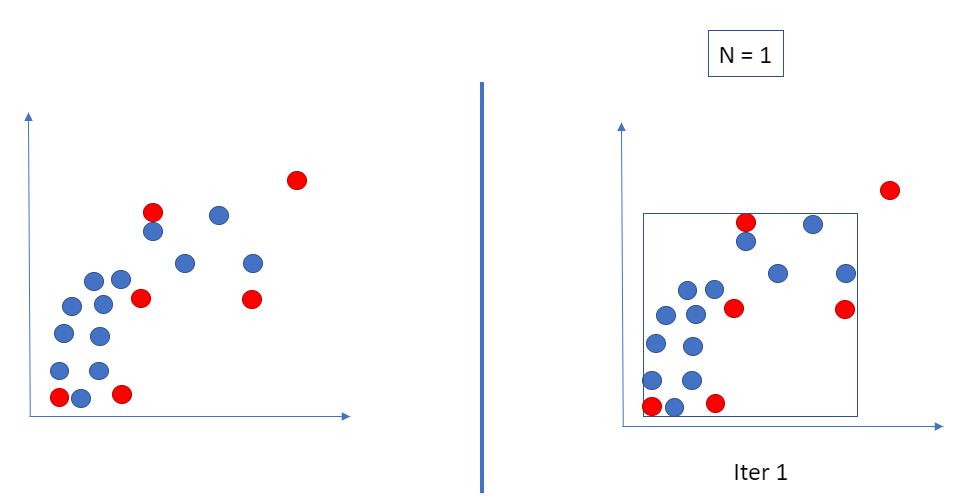
\includegraphics[width=0.7\columnwidth]{figures/chapter4_RuleExtraction/start.png}
  \end{tabular} 
  \caption{Clustering over a 2D space. With one cluster over data points from one class (blue), there are still others from the other class (red) inside the square.\label{fig:ch4-starting-point}}
\end{figure}

\begin{figure}[!h]
\centering
  \begin{tabular}{c@{\qquad}c@{\qquad}c}
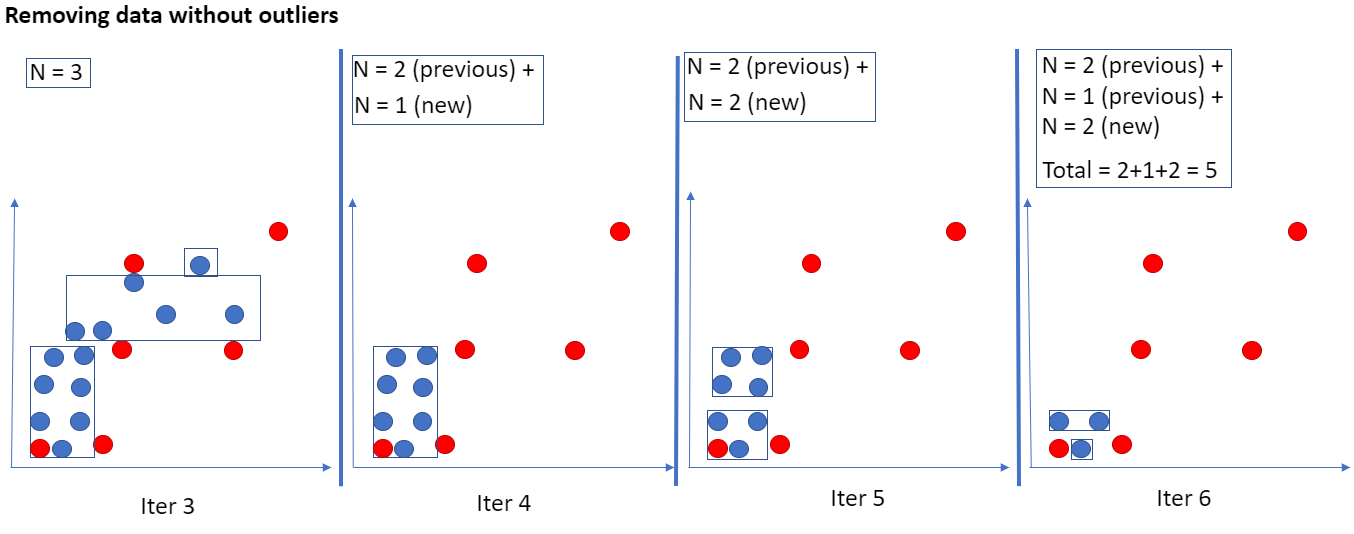
\includegraphics[width=0.8\columnwidth]{figures/chapter4_RuleExtraction/discard.png}
  \end{tabular} 
  \caption{Applying the proposal of \parencite{nunez2002rule}, the number of clusters keeps increasing until no points from the other class are inside, an then that hypercube is translated into a rule.\label{fig:ch4-discard}}
\end{figure}

The approximation proposed before is not the only one that can be applied in order to extract the rules. \hyperref[fig:ch4-keep]{Figure} \ref{fig:ch4-keep} shows one of our alternative proposals over \parencite{nunez2002rule} method. Instead of removing data points that are inside a rule without points from the other class, the process always keeps all data points in every iteration since there could be clustering patters that could only be found if all points are together. In this approach, the number of clusters is constantly increased until no data points from the other class are inside the hypercubes, or the maximum number of iterations is reached. We will further address this method as \textbf{keep} in the remaining of the chapter. In contrast, the references to \parencite{nunez2002rule} method will be addressed as \textbf{keep\_reset}.

\begin{figure}[!h]
\centering
  \begin{tabular}{c@{\qquad}c@{\qquad}c}
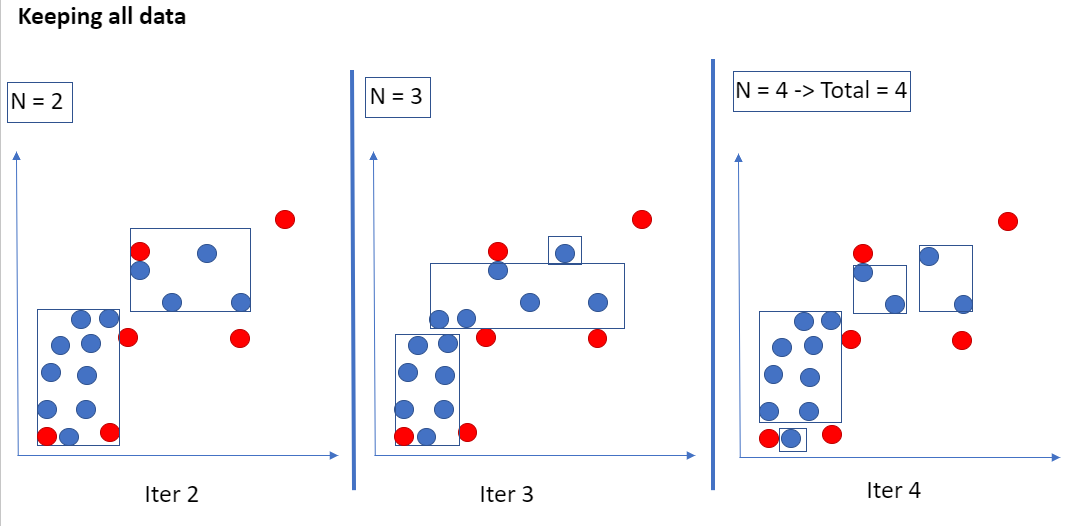
\includegraphics[width=0.75\columnwidth]{figures/chapter4_RuleExtraction/keep.png}
  \end{tabular} 
  \caption{Keeping all data points in every iteration could lead to a reduced number of clusters since there may be data patterns that could only be found in this scenario. \label{fig:ch4-keep}}
\end{figure}

Another proposal that we include in this chapter over \parencite{nunez2002rule} is splitting the subspaces in a binary partition scheme. This is an alternative over the original proposal, that constantly increases the number of clusters until one rule has only data points from the same class, and then restarting the clustering process from the beginning for the remaining ones. We will address this method as \textbf{split} for the remaining of the chapter. \hyperref[fig:ch4-keep-reset]{Figure} \ref{fig:ch4-keep-reset} shows how the same 2D example using this approach.

\begin{figure}[!h]
\centering
  \begin{tabular}{c@{\qquad}c@{\qquad}c}
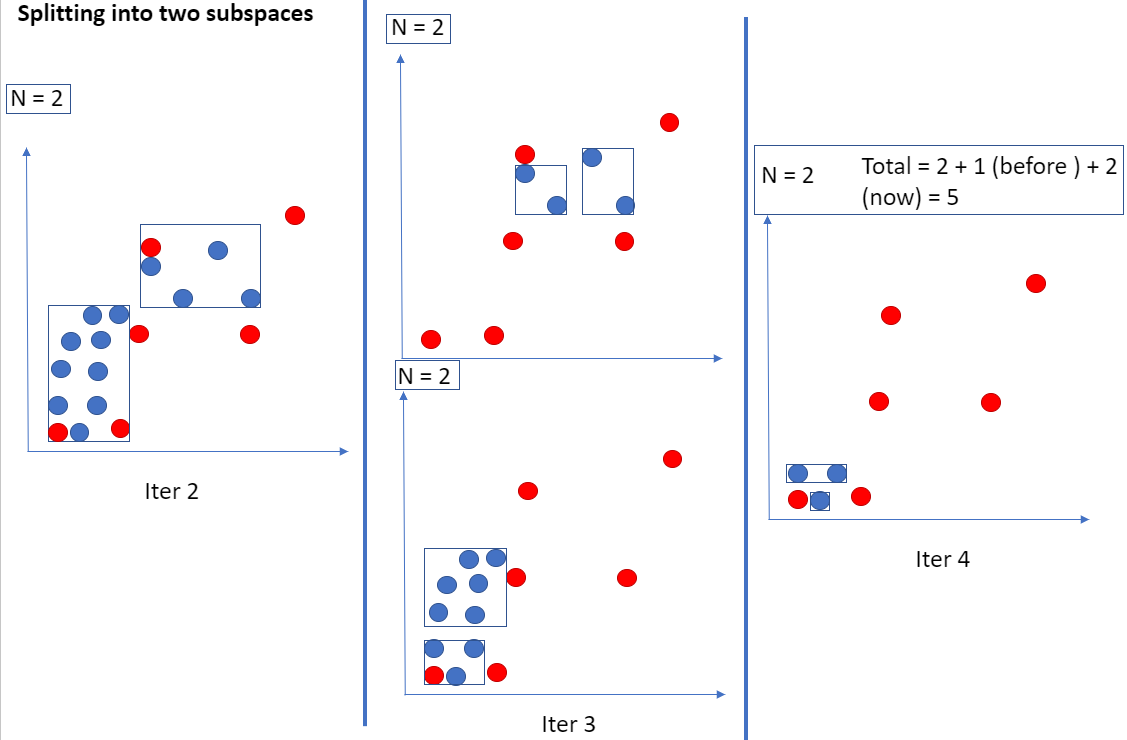
\includegraphics[width=0.7\columnwidth]{figures/chapter4_RuleExtraction/keep_reset.png}
  \end{tabular} 
  \caption{Splitting subspaces with a binary partition scheme until no red points are inside the rule. \label{fig:ch4-keep-reset}}
\end{figure}

According to the taxonomy for XAI in \parencite{molnar2019interpretable}, our method has the following characteristics:
\begin{itemize}
    \item \textbf{Post-hoc}: Explainability is achieved using external techniques.
    \item \textbf{Global and individual}: Explanations serve to explain how the whole model works, as well as why a specific data point is considered anomalous or non-anomalous.
    \item \textbf{Model-agnostic}: As with other techniques for global explanations \parencite{molnar2019interpretable}, the only information needed to build the explanations are the input features and the outcomes of the system after fitting the model.
    \item \textbf{Counterfactual}: The explanations for why a data point is anomalous also include information on the changes that should take place in the feature values in order to consider that data point as non-anomalous.
\end{itemize}

Since the explanation algorithm is model-agnostic, it can work for any blackbox model. The only information needed is the train data set and the outputs from the model.  To illustrate it, we show evaluations over OCSVM models with different kernels: radial basis function (RBF) and linear kernel.

Regarding the clustering technique itself, potentially any algorithm could be used, both for \parencite{nunez2002rule} or for any of out two proposals over it from this chapter. However, there is a caveat that should be considered. The clustering algorithm needs to take into account if the features are only numerical, categorical (non ordinal), or both. 

One algorithm that will be used in this chapter for extracting the hypercubes is K-Means ++ \parencite{arthur2006k}. However, the standard version of this clustering algorithm is designed for numerical features, and categorical ones should be treated differently. In that case, the approximation would be to extract a rule for each of the possible combinations of categorical values among the data points that are not considered anomalous. Considering again the aforementioned 2-dimensional example, with variable X being binary categorical, a data set may look like in \hyperref[fig:ch4-outlier5]{Figure} \ref{fig:ch4-outlier5}:

\begin{figure}[h!]
\centering
  \begin{tabular}{c@{\qquad}c@{\qquad}c}
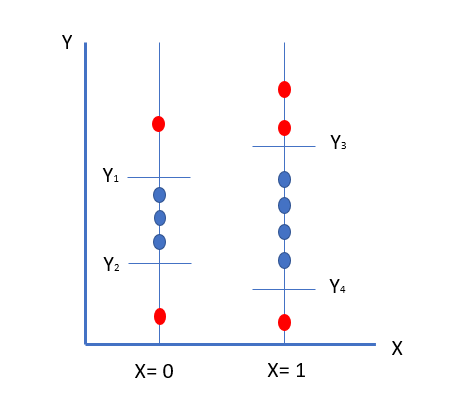
\includegraphics[width=0.50\columnwidth]{figures/chapter4_RuleExtraction/outlier_05.png}
  \end{tabular} 
  \caption{Rule extraction with a categorical variable.\label{fig:ch4-outlier5}}
\end{figure}

In that case, two rules would be extracted, one for each of the possible states of X:
\begin{itemize}
    \item Rule 1: NOT OUTLIER IF X = 0 $\land$ Y $\geq$ Y2 $\land$ Y $\leq$ Y1
    \item Rule 2: NOT OUTLIER IF X = 1 $\land$ Y $\geq$ Y4 $\land$ Y $\leq$ Y3
\end{itemize}

Generally speaking, the algorithm logic can be summarised as:
\begin{itemize}
    \item Apply OCSVM to the data set to create the model.
    \item Depending on the characteristics of variables, do:
    \begin{itemize}
    \item \underline{Case 1. Numerical only}:  Iteratively create clusters in the non-anomalous data (starting with one cluster) and create a hypercube using the centroid and the points further away from it. Check whether the hypercube contains any data point from the anomalous group; if it does, repeat using one more cluster than before. Finish when no anomalies are contained in the generated hypercubes. If there are anomalies and the data points in a cluster are inferior to the number of vertices needed for the hypercube, complete the missing vertices with artificial data points and finish when there are no anomalies or when the convergence criterion is reached.
    \item \underline{Case 2. Categorical only}: The rules will correspond directly to the different value states contained in the data set of non-anomalous points.
    \item \underline{Case 3. Both numerical and categorical}. This case would be analogous to Case 1, but data points will be filtered for each of the combinations of the categorical variables states. For each combination, there will be a set of rules for the numerical features.
    \end{itemize}
    \item Use these vertices to obtain the boundaries of that hypercube and directly extract rules from them.
\end{itemize}

Besides K-Means++, there are other clustering algorithms that may be applied. We will analyse also the rules obtained by applying K-Prototypes \parencite{ji2013improved}. The advantage of using K-Prototypes is that it can work directly with both categorical and numerical features.

The algorithms described within this section correspond to the two alternative methods within the \textbf{TC1 SVM+Prototypes reloaded} algorithm, which was introduced within \hyperref[sec:Hypotheses]{Section} \ref{sec:Hypotheses}.

\section{XAI metrics for rule extraction techniques}\label{sec:RuleExtractionMetrics}
In this section, we describe the different XAI metrics that we propose for assessing and comparing the quality of rule-based explanations. The metrics that we consider are divided into four subsets: \textit{comprehensibility}, \textit{representativeness}, \textit{stability} and \textit{diversity}. The reason behind it is that, to the best of our knowledge, some of these metrics do not have an algorithm implementation for the context of rule extraction techniques (they are only defined in a general way). This is the case of \textit{stability} and \textit{diversity}. The remaining metrics are chosen because they are relevant within the literature, and for the particular case of \textit{representativeness}, there are no frameworks that implement them within the context of P@k rules. 

We propose how to compute these metrics within this section, and we evaluate them over the case of unsupervised anomaly detection using OCSVM models. However, they could be applied for any model that has a binary output and that is explained through rule extraction techniques.

\begin{itemize}
    \item \textbf{Metrics for comprehensibility}: Number of rules ($nRules$), size of the rules ($sizeRules$).
    \item \textbf{Metrics for representativeness}: Percentage of data points explained with P@1 rules ($perP1$) and the median percentage coverage of data points by each rule ($p1Coverage$).
    \item  \textbf{Metrics for stability}: How many artificial points (similar to a subset of prototypes from the data set) are classified by the rules with the same predictions yielded by original blackbox model ($StabilityScore$).
    \item \textbf{Metrics for diversity}: Metric based on the degree of hyperspace overlapping between all the rules ($DiversityScore$).
\end{itemize}

\subsection{Metrics for comprehensibility}\label{subsec:RuleExtractionComprehensibility}
The metrics for \textit{comprehensibility} are directly analyzed from the rules themselves; $nRules$ is computed counting the number of rules generated, and $sizeRules$ is computed checking the elements that define the rule (i.e. $X > 3$ AND $X < 7$ AND $Y > 1$ have a $sizeRules=3$ while $X > 3$ have a $sizeRules=1$). This proposal already appears in \parencite{barakat2010rule}.

\subsection{Metrics for representativeness}\label{subsec:RuleExtractionRepresentativeness}
The metric $perP1$ for \textit{representativeness} simply checks the percentage of data points for the target class explained with P@1 rules. The other metric in this group is $p1Coverage$. It checks the median performance of the rules themselves: it computes the median percentage of coverage for the target class by each rule. These proposals are similar to \parencite{vilone2020comparative}, with the particularity of focusing on P@1 rules. We defined P@1 specifically, but it can be extended for other P@k thresholds.

\subsection{Metrics for stability}\label{subsec:RuleExtractionStability}
The metric $StabilityScore$ computes the \textit{stability} metric of the hypercubes. The first step is obtaining the prototypes from the data set and generate random samples near them. Then, obtain the prediction of the original model for those artificial samples and checks if the predictions using the rules are the same.

The steps for these metric are described below, and the detailed pseudocode appears in \hyperref[alg:ch4-stability]{Algorithm} \ref{alg:ch4-stability}. 

Model agreement:
\begin{itemize}
    \setlength{\itemindent}{2em}
    \item Choose N prototypes that represent the original hyperspace of data
    \item Generate M samples close to each of those N prototypes using Protodash algorithm \parencite{gurumoorthy2019efficient}; the hypothesis is that close points should be generally predicted belonging to the same class.
    \item For each of those N*M data points (M data points per each N prototype) check whether the rules (all of them) predict them as inliner or outlier; the data points that come into the function are either outliers or inliers. If they are inliers,  then the rules identify an artificial data point (of those M*N) as inlier if it is outside every rule. If the data points are outliers it's the same reversed: a data point is an inlier if no rule includes it.
    \item It then checks if the predictions using the rules for those artificial data points are the same as the one provided by the original model.
    \item With that, it computes \% of predictions for the artificial data points aforementioned that are the same between the rules and the original OCSVM model.
\end{itemize}

\hyperref[alg:ch4-stability]{Algorithm} \ref{alg:ch4-stability} receives the data set $X$ of inliers/outliers (depending if the rules are computed for inliers or outliers), the rules $X_r$ and the OCSVM fitted and trained model $clf$. Then obtains the protoypes with $ProtodashExplainer()$ function and generates the random samples $X_s$ near them with $randomNear()$, where an upper and lower limits ($th_s$, $th_l$) can be defined for how close are those points to the prototypes. Then, it checks which rules enclose that data point with $checkInR()$, and if at least one of them encloses the data point, it is considered that it can be classified using the rules. The metric $StabilityScore$ is specified in $n\_precision$ variable, that checks the percentage of agreement between the classifications using the rules and the ones with the model, through $checkInModel()$ function. 

\begin{algorithm}[h!]
\caption{StabilityScore}\label{alg:ch4-stability}
\begin{algorithmic}[1]
\Procedure{getAgreement}{$X, X_r, clf$}
    \State $X_p \gets ProtodashExplainer(X)$
    \State $X_s \gets []$
    \For{$p\in X_p$}
        \State $X_s \gets X_s.append(randomNear(p, th_l, th_s))$
    \EndFor\label{generate_samples}
    \State $n\_precision \gets 0$
    \State $l\_rules \gets []$
    \For{$d\in X_s$}
        \State $l\_iter \gets []$
        \For{$r\in X_r$}
             \State $l\_iter \gets l\_iter.append(checkInR(d, r))$
        \EndFor
        \State $r\_rules \gets max(l\_iter)$
        \State $r\_model \gets checkInModel(d, clf)$
        \If{$r\_rules = r\_model$}
            \State $n\_precision \gets n\_precision+1$
        \EndIf\label{compute_agreement}
       % \State $l\_rules \gets l\_rules.append(r\_rules)$
    \EndFor
    \State $n\_precision \gets n\_precision/len(X_s)$
    %\State $n\_agreement \gets l\_rules[=1]/len(X_s)$
    %\State \textbf{return} $n\_precision, n\_agreement$
    \State \textbf{return} $n\_precision$
\EndProcedure
\end{algorithmic}
\end{algorithm}

\hyperref[alg:ch4-stability]{Algorithm} \ref{alg:ch4-stability} corresponds to \textbf{TC2 StabilityScore}, which was introduced within \hyperref[sec:Hypotheses]{Section} \ref{sec:Hypotheses}.

Additionally, a proof that StabilityScore is a metric is included in \hyperref[sec:annex-demonstration-metric-stability]{Subsection} \ref{sec:annex-demonstration-metric-stability} within the \hyperref[ch:annex]{Annex}.

\subsection{Metrics for diversity}\label{subsec:RuleExtractionDiversity}
The metric to measure \textit{diversity} is $DiversityScore$, and it analyses if the rules are different with few overlapping concepts. This is computed checking the area of the hypercubes of the rules that overlaps with another one.
The way to check this is by seeing the 2D planes of each hypercube (by keeping two degrees of freedom for the features in the hyperplane coordinates; n-2 features are maintained and the other two are changed between their max/min values in order to obtain the vertices of that 2D plane). Then, it obtains the area of the 2D planes for the rules that overlaps, and each of those 2D areas is turned into a score between 0 and 1 by using the Jaccard similarity index and dividing the area of intersection of the 2D planes by their area of union.

The pseudocode for this metric appears in \hyperref[alg:ch4-score-intersect]{Algorithm} \ref{alg:ch4-score-intersect}. It receives the data set $X$ of inliers/outliers (depending if the rules are computed for inliers or outliers), the rules $X_r$, the list of columns for numerical features $l\_n$ and the one for categorical $l\_c$.
The first step is obtaining all the two tuples combinations of numerical features, using $combinations()$ function. After that, it obtains the combination of categorical values with function $unique()$. The algorithm then analyses separately the rules that belong to each categorical combination values. For each of those subset of rules $X\_r\_i$, if there are at least two rules, then it defines the tuples of possible rule combinations, $combR$. Then, it iterates per each combination of two numerical features. These two features will correspond to the features that will be changed, leaving the rest of the $l\_fix$ features fixed, in order to extract 2D planes from the hypercubes with $get2D$, and storing those planes in $polys$ variable. Those planes are used for obtaining the Jaccard similarity index with $scorePolys()$ function. If there is an iteration where one of the two dimensions has the same value, it is skipped since the area will be 0. ($checkEqual(pair_f)$).

\hyperref[fig:ch4-img-cubes]{Figure} \ref{fig:ch4-img-cubes} describes the process for an example in a 3D space. Since all the rules translate into a hypercube, we can choose two features at a time (leaving the rest fixed) and obtain the coordinates for those 2D planes (using their vertices values). Then, for two rules, we can see the area of overlapping between those 2D hyperplanes, as well as their area of union. With that areas, we obtain the Jaccard similarity index. Since the Jaccard similarity index ($score\_i$) yields a value between 0 and 1 (0 when there is no overlapping, and 1 when the area of intersection is the same as the area of union in a total overlapping), we can turn it into a metric in order to express a score value by doing $1-score\_i$, so a perfect score will be the one corresponding to no overlap between the rules. This is repeated for all 2D planes of the hypercubes, and we compute the mean of all the individual scores in order to have one final metric ($final\_score$) that is still between 0 and 1, with 1 the perfect score and 0 the worst.

\begin{figure}[h!]
\centering
  \begin{tabular}{c@{\qquad}c@{\qquad}c}
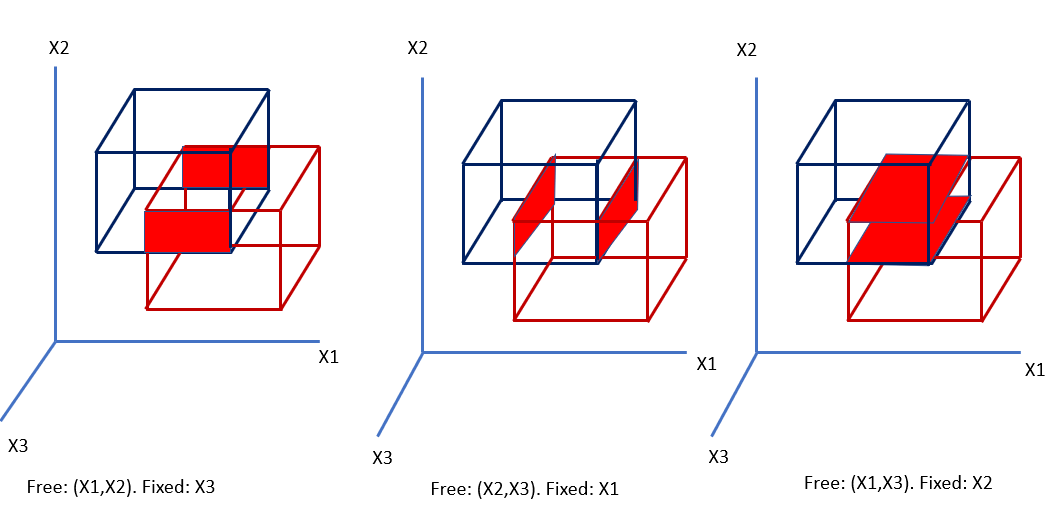
\includegraphics[width=0.8 \columnwidth]{figures/chapter4_RuleExtraction/img_cubes.png}
  \end{tabular} 
  \caption{The overlapping between rules (hypercubes) approximated using their 2D planes' area of intersection.\label{fig:ch4-img-cubes}}
\end{figure}

\begin{algorithm}[h!]
\caption{DiversityScore}\label{alg:ch4-score-intersect}
\begin{algorithmic}[1]
\Procedure{getInterScore}{$X, X\_r, l\_n, l\_c$}
    \State $l\_free \gets combinations(l\_n, 2)$
    \State $X\_c \gets unique(X[l\_c])$
    \State $score \gets []$
    \State $n\_inter \gets 0$
    \For{$cat \in rows(X\_c)$}
        \State $X\_r\_i \gets X\_r[cat]$
        \If{$len(X\_r\_i)>2$}
            \State $combR \gets combinations(X\_r\_i, 2)$
            \For{$pair_f \in l\_free$}
                \If{$checkEqual(pair_f)$}
                \State $continue$
                \EndIf
                \State $l\_fix \gets l\_n[!=pair_f]$
                \State $polys \gets get2D(combR, l\_fix,pair_f)$
                \State $score\_i, n\_i \gets scorePolys(polys)$
                \State $score \gets score.appends(1 - score\_i)$
                \State $n\_inter \gets n\_inter + n\_i$
            \EndFor
        \EndIf
    \EndFor
    \State $final\_score \gets mean(score)$
    \State \textbf{return} $final\_score$
\EndProcedure
\end{algorithmic}
\end{algorithm}

All the algorithms that we have proposed for computing XAI metrics are \textit{XAI-specific metrics}: metrics that are specific for a particular type of XAI technique (in this case, rule extraction).

\hyperref[alg:ch4-stability]{Algorithm} \ref{alg:ch4-stability} corresponds to \textbf{TC3 DiversityScore}, which was introduced within \hyperref[sec:Hypotheses]{Section} \ref{sec:Hypotheses}.

Additionally, a proof that DiversityScore is a metric is included in \hyperref[sec:annex-demonstration-metric-diversity]{Subsection} \ref{sec:annex-demonstration-metric-diversity} within the \hyperref[ch:annex]{Annex}.

\subsection{Towards one metric for summarizing all of them}\label{subsec:RuleExtractionOneMetric}
There is a question that will arise at this point: Which rule would be better? One with better results in \textit{comprehensibility}, or one with better results at, for instance, \textit{diversity}? When there is a need to choose a trade-off, which criteria should be prioritized? 
The answer to this will heavily depend upon the domain needs. However, in general terms, all the metrics can be combined into a single one that offers a unique view over them. It can be done with a metric in terms of $final\_metric = f(C, R, S, D)$ with C representing the comprehensibility metrics, R the representativeness, S the stability and D the diversity. There is another aspect that can be considered while creating a function to encapsulate all metrics. In general, it is better to have a lower value for comprehensibility metrics (less rules, less rule size) since that may contribute to an enhancement of comprehensibility. Regarding the rest of the metrics, higher values are better. Thus, a simple way to compute this is adding the results for representativeness, stability and diversity (adjusting their relative importance by a set of weights), and subtracting comprehensibility results. Since the values for the metric of comprehensibility are the only ones that are not in a range of 0 to 1, we scale them before computing this metric in order to have all values in the same range. This is done by dividing them with respect to the number of inliers or outliers (number of rules) or by a value based on the number of features (rule size).

With this, a higher final value will be better. This is expressed in \hyperref[eq:ch4-finalmetric]{Equation} \ref{eq:ch4-finalmetric}.

\begin{equation}\label{eq:ch4-finalmetric}
\begin{split}
  C = {\alpha_1 * (1 - nRules) + \alpha_2 * (1 - sizeRules)} \\
  R = \beta_1 * perP1 + \beta_2 * p1Coverage \\
  S = \gamma*StabilityScore \\
  D = \theta*DiversityScore \\
  final\_metric = \frac{(R + S + D + C)}{N} \\
\end{split}
\end{equation}
\myequations{Rule proposal: Final metric}

$N$ equals to the number of metrics considered (6 in this case). The different $\alpha$, $\beta$, $\gamma$ and $\theta$ parameters could be adjusted in order to weight the different metrics in case one of them is more important than others. Our proposed methods to compute a general metric is a very naive way to approach it, and more sophisticated ways could be explored. However, its important to highlight the need to be able to analyse everything together for some use cases, since there are many XAI aspects to measure and it may difficult to perform a comparison between XAI techniques.

\hyperref[eq:ch4-finalmetric]{Equation} \ref{eq:ch4-finalmetric} corresponds to \textbf{TC4}, which was introduced within \hyperref[sec:Hypotheses]{Section} \ref{sec:Hypotheses}.

\section{A framework for extracting and evaluating rule-based explanations}\label{sec:RuleExtractionFramework}
In this section, we describe our proposed general framework, \textbf{HyperRulEx} (\textbf{Hyper}cube \textbf{Rule} \textbf{Ex}traction), that standardizes rule extraction techniques, optimizes them, and obtains XAI specific metrics for assessing and comparing the quality of the explanations.

\subsection{Framework description}\label{subsec:RuleExtractionFramework}
The general flowchart followed by the framework appears in \hyperref[fig:ch4-flowchartRULEX]{Figure} \ref{fig:ch4-flowchartRULEX}. The first step applies a unsupervised ML algorithm for anomaly detection, yielding a binary output identifying the registers that are inliers and those that are outliers. Then, it applies a post-hoc rule extraction XAI algorithm that extracts the explanations. After that, the explanations are standardized by turning them into hypercubes, as exemplified in 
\hyperref[fig:ch4-format-not-homog]{Figure} \ref{fig:ch4-format-not-homog}. Then, after obtaining the hypercubes, the next step prunes the rules, eliminating those that are encapsulated by another bigger one. This step is described in more detail at \hyperref[subsec:RuleExtractionPruning]{Subsection} \ref{subsec:RuleExtractionPruning}. After that, it applies the XAI metrics \hyperref[sec:RuleExtractionMetrics]{Section} \ref{sec:RuleExtractionMetrics} for explanation evaluation. Even though our study focuses on XAI metrics that do not require a ground truth for the evaluation, the framework can be extended for including an evaluation against that ground truth both with specific XAI metrics as well as with model performance ones (e.g. F1).

\begin{figure}[h!]
\centering
  \begin{tabular}{c@{\qquad}c@{\qquad}c}
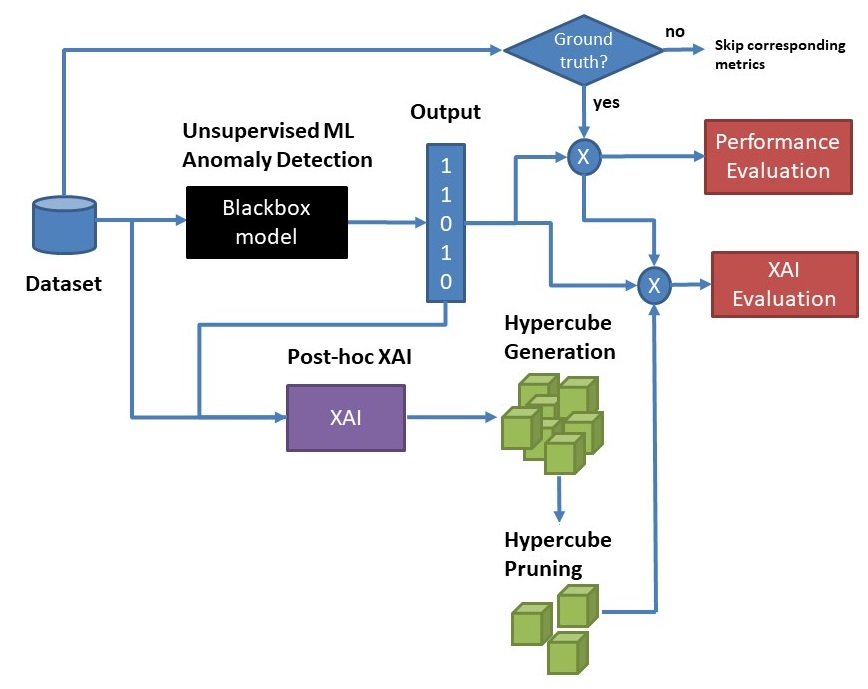
\includegraphics[width=0.80\columnwidth]{figures/chapter4_RuleExtraction/flowchartRULEX_notitle.jpg}
  \end{tabular} 
  \caption{Flowchart of the proposed framework that standardizes rule extraction XAI methods, optimizes the results and evaluate the final explanations with XAI  metrics.\label{fig:ch4-flowchartRULEX}}
\end{figure}


\begin{figure}[h!]
\centering
  \begin{tabular}{c@{\qquad}c@{\qquad}c}
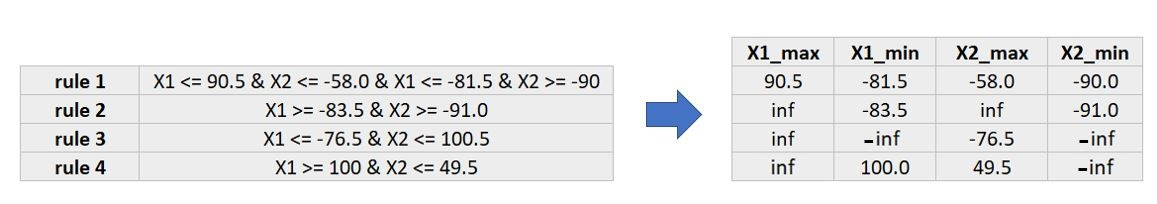
\includegraphics[width=0.95\columnwidth]{figures/chapter4_RuleExtraction/RuleFormatNotHomog4.JPG}
  \end{tabular} 
  \caption{Example showing the output of a rule extraction XAI algorithm over a sample case where there are only two input features. Left side shows the original rules yielded, where there are instances with redundant elements. Right side shows the hypercube (square in this case), corresponding to the transformed rules.\label{fig:ch4-format-not-homog}}
\end{figure}


\subsection{Pruning rules}\label{subsec:RuleExtractionPruning}
Many of the rules obtained with all the methods described above are suboptimal, since they can be enclosed into another bigger rule. In order to reduce the number of rules, and remove redundancies, we apply a simple pruning technique prior to the computing and evaluation of metrics.
We check every hypercube generated and see if their limits are inside any other rule. If they are, we eliminate that rule from the set of rules. We check this for every rule against every other rule in the data set, and we keep checking it in a loop until no rules are eliminated, until we reach a fixed point.

\section{Evaluation}\label{sec:RuleExtractionEvaluation}
This section presents the evaluation of hypothesis \textbf{H1} (described in \hyperref[sec:Hypotheses]{Section} \ref{sec:Hypotheses}) considering our proposal. The metric proposals described in \hyperref[sec:RuleExtractionMetrics]{Section} \ref{sec:RuleExtractionMetrics} serve directly as a justification for evaluating the hypothesis, since we provide a mathematical justification for these metrics. Nonetheless, we want to complement it by using our proposal over several data sets, applying the metrics for analysing the explanations obtained. With that, we want to show how the metrics are useful for finding out rule extraction techniques that are more suitable than others for a specific context (unsupervised anomaly detection with P@1 rules in this case), even if all those methods are post-hoc and model-agnostic. Because of that, we define several sub-hypotheses during this evaluation which serve as a reinforcement for checking \textbf{H1}.

In particular, we evaluate our proposal over data sets (both public and from Telefonica's real data), for assessing these following sub-hypotheses:
\begin{itemize}
    \item \textbf{Sub-hypothesis 1 (SH1):} The rule extraction method of \parencite{nunez2002rule} and our proposed variations applied over OCSVM for anomaly detection using a RBF kernel yield significantly less P@1 rules when applied for explaining inliers than for outliers or when using a linear kernel. \label{subhypothesis:subhypothesis4_1}
    \item \textbf{Sub-hypothesis 2 (SH2):} Our proposed variations over \parencite{nunez2002rule} yield similar results for P@1 rules that explain the inliers of an OCSVM anomaly detection model when compared to \parencite{nunez2002rule} in terms of explainability regardless of the kernel (considering Linear and RBF). \label{subhypothesis:subhypothesis4_2}
    \item \textbf{Sub-hypothesis 3 (SH3):} The rule extraction method of \parencite{nunez2002rule} and our proposed variations yield better results for P@1 rules that explain the inliers of an OCSVM anomaly detection model in terms of explainability than other rule extraction techniques and regardless of the kernel (considering Linear and RBF). \label{subhypothesis:subhypothesis4_3}
\end{itemize}

Explanations in terms of rule extraction for anomaly detection may help to see with a counterfactual view what would make an outlier turn into an inlier by explaining the inlier class (for local explanations). For explaining what feature values are normally associated with outlier data points (global explanations), these explanations will target the outlier class. This is why \textit{SH1} checks the contribution of RBF kernel for grouping data points inside its hypersphere in order to help explaining them with less rules.

For the hypothesis checks, we consider the results yielded by the XAI rule extraction methods over different data sets (\hyperref[subsec:RuleExtractionDataSets]{Section} \ref{subsec:RuleExtractionDataSets}), together with the type of kernel used for the OCSVM, as well as the type of data points explained (outliers or inliers). Thus, we have N data sets x 2 types of kernel x 2 types of data points. This serves for performing an hypothesis contrast based on the Wilcoxon signed-rank test \parencite{conover1998practical}, since it has been proved useful for comparing different ML model metrics results over several data sets for both classification \parencite{demvsar2006statistical} and regression tasks \parencite{trawinski2012nonparametric}.

The code is available for reproducibility through our published paper \parencite{barbado2022rule} or directly within the repository \parencite{Barbado2019}. The specific libraries and model configurations are detailed in \hyperref[sec:annex-rule-extraction-config]{Subsection} \ref{sec:annex-rule-extraction-config} within the \hyperref[ch:annex]{Annex} \ref{ch:annex}.

\subsection{Data sets}\label{subsec:RuleExtractionDataSets}
The data sets that we have used for evaluation belong to different domains, have different sizes and different number of features (both categorical and numerical), as indicated in \hyperref[table:ch4-rule-extraction-datasets]{Table} \ref{table:ch4-rule-extraction-datasets}:
\begin{itemize}
%    \setlength{\itemindent}{2em}
    \item Data sets 1 and 2 are about seismic activity \parencite{sathe2016lodes}. data set 1 is bi-dimensional with only numerical features ('gdenergy', 'gdpuls'). data set 2 has 2 categorical features ('hazard', 'shift') and 7 numerical ('seismoacoustic', 'shift', 'genergy', 'gplus', 'gdenergy', 'gdpuls', 'hazard', 'bumps', 'bumps2').
    \item Data set 3 is about cardiovascular diseases \parencite{padmanabhan2019physician}. There are 4 categorical features ('smoke', 'alco', 'active', 'is\textunderscore man') and 7 numerical ('age', 'height', 'weight', 'ap\textunderscore hi', 'ap\textunderscore lo','cholesterol','gluc').
    \item Data set 4 is from a call center at Telefónica (TEF Comms) \parencite{patent2019comms}. It is real data that includes the total number of calls received in one of its services during every hour. Using these data, some features are extracted (weekday), and they are cyclically transformed, so that each time feature turns into two features for the sine and cosine components. The rules in this case are also transformed back into the original features in order to enhance rule comprehension. 
    \item Data set 5 contains Telefónica's data about IoT devices attached to cars for vehicle tracking \parencite{patent2020fleet}. The data is aggregated in daily windows for each vehicle, representing features that model the daily behaviour of that vehicle. It contains 49 numerical features (such as the number of events with high RPM or the maximum temperature of the coolant), and 12 categorical ones (binary variables that indicate the model and make of that car, among others).
    \item Data set 6 refers to United States census for year 1990 \parencite{blake1998uci}. It has 2 categorical features ('dAncstry1\textunderscore 3', 'dAncstry1\textunderscore 4') and 7 numerical ones ('dAge', 'iYearsch', 'iFertil', 'iImmigr', 'iYearwrk', 'dTravtime', 'dRearning').
\end{itemize}

\begin{table}[h!]
\centering
\begin{tabular}{lllll} 
 \textbf{Data set} & \textbf{Ref.} & \textbf{Nº Cat.} & \textbf{Nº Num.} & \textbf{Nº Rows} \\ [0.5ex]
 \hline
 D1 & \parencite{sathe2016lodes} & 0 & 2 & 669\\ 
 D2 & \parencite{sathe2016lodes} & 2 & 7 & 1705\\
 D3 & \parencite{padmanabhan2019physician} & 4 & 7 & 42000\\
 D4 & \parencite{patent2019comms} & 0 & 5 & 2712\\
 D5 & \parencite{patent2020fleet} & 12 & 49 & 59844\\
 D6 & \parencite{blake1998uci} & 2 & 7 & 106819\\  [1ex]
\end{tabular}
\caption{Description of each data set, with their reference (Ref.), categorical features (Nº Cat.), numerical features (Nº Num) and number of rows.}
\label{table:ch4-rule-extraction-datasets}
\end{table}

\subsection{Results}\label{subsec:RuleExtractionResults}
In this subsection we describe the evaluation of our hypotheses. We will refer to K-Means approach as KM, and K-Prototypes as KP. Thus, for instance, K-Means with the "split" method will be identified as KM\_split.

% Hypothesis 1
\hyperref[table:annex-rule-extraction-hypothesis1]{Table} \ref{table:annex-rule-extraction-hypothesis1} provides the \textbf{results associated to \textit{\hyperref[subhypothesis:subhypothesis4_1]{SH1}}}. Here, we want to check if there are significantly less P@1 rules for inliers using a RBF kernel, compared to using a linear kernel for inliers, or the same RBF kernel for outliers. For the Wilcoxon signed-rank tests we only compare combinations of method-kernel-inliers/outliers for data sets that have at least 1 P@1 rule. Since the comparisons involve few data points in some cases, we check against a minimum p-value of 0.1. Considering this, only KM\_split and KM\_keep have significant differences in the number of rules. In those cases, H1 is actually rejected: RBF for inliers yields more rules than either RBF for outliers, or linear for inliers. Regarding the other methods, there are no statistically strong results to conclude anything. With that, even though it is not assured for every method, \textbf{these rule extraction methods when applied to inliers and when using a RBF kernel tend to generate more rules than in the other cases}.

% Hypothesis 2
After comparing those rule extraction methods in terms of the number of rules in order to see significant differences depending on the type of data points (inliers/outliers) and the type of kernel (RBF/linear), we proceed to check \textbf{\textit{\hyperref[subhypothesis:subhypothesis4_2]{SH2}}}. Here, we compare the methods considering all the XAI metrics proposed previously. This is done by checking every metric over every combination of data set, kernel and type of data (inliers/outliers), and performing a Wilcoxon signed-rank test in order to see if there are no significant differences between the methods for each of the metrics. Since the data points in this case are superior than those present at \textit{SH1}, we check against a minimum p-value of 0.05. For \textit{SH2}, there is no need to check the size of the rules since they will be the same for all the methods using K-Means and for all the methods using K-Prototypes. We only compare between data sets-kernel-type of data that exists in both methods considered. Thus, the means for the KM methods may vary depending on whether they are compared between them or they are compared against KP ones (and vice versa). 

At \hyperref[table:annex-rule-extraction-hypothesis1]{Table} \ref{table:annex-rule-extraction-xai-metrics-h2}, we see the methods and metrics that have significant differences according to Wilcoxon signed-rank test. There are some cases where the metrics do differ significantly, as some methods yield better results. \textbf{KM\_split method outperforms every other one regarding the percentage of data points covered by its P@1 rules (per\_p1). It does so in exchange of yielding a greater number of rules than some of the other methods, like KM\_keep\_reset}. Thus, it increases \textit{representativeness} by losing in terms of \textit{comprehensibility}. In general, KM methods cover more data points with P@1 rules that their counterparts with KP. Considering the other metric from \textit{representativeness}, p1\_coverage, there are no significant differences between KM\_split and KM\_keep\_reset, but both methods yield better results than KM\_keep. Thus, usually the P@1 rules that they yield are able to cover more data points. This is logical, since the algorithm that yields the rules in the case of KM\_keep tends to generate smaller hypercubes. An example of this can be seen in \hyperref[fig:ch4-evaluation-img-clustering-2D]{Figure} \ref{fig:ch4-evaluation-img-clustering-2D} for data set D1. We can see how KM\_keep indeed yields rules that are smaller than the ones from the other methods.  

\begin{figure}[h!]
\centering
  \begin{tabular}{c@{\qquad}c@{\qquad}c}
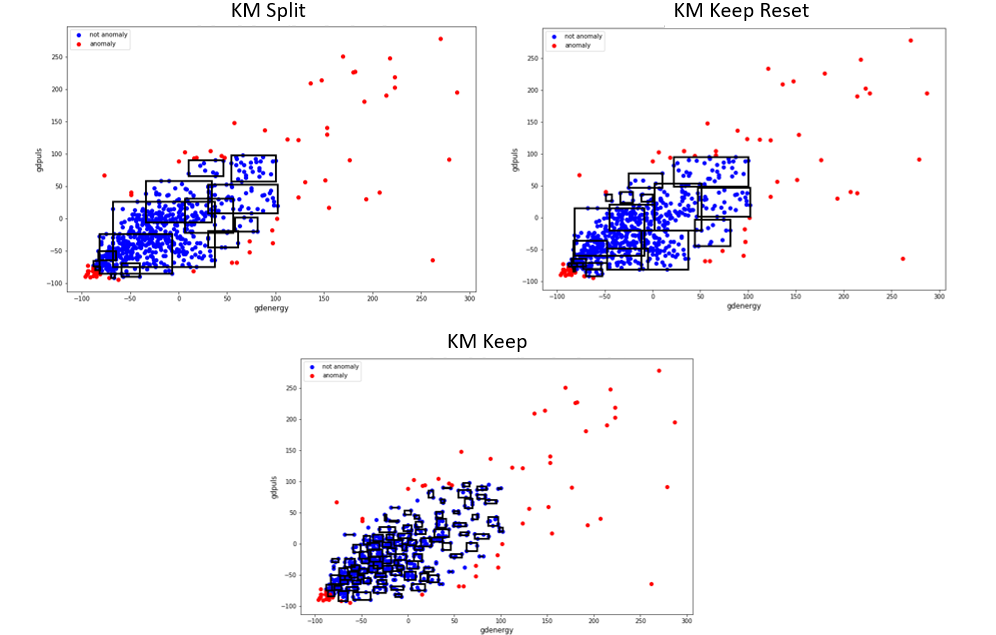
\includegraphics[width=0.9 \columnwidth]{figures/chapter4_RuleExtraction/clusteringMethods_comparison.PNG}
  \end{tabular} 
  \caption{K-Means based rule extraction methods (for inliers) over D1 data set with RBF kernel. \label{fig:ch4-evaluation-img-clustering-2D}}
\end{figure}

Regarding \textit{representativeness} (DiversityScore), there are no significant differences between KM methods, but all of them outperform all the KP ones. In terms of \textit{stability} (StabilityScore), we see no significant difference between any of the methods.
Finally, the general metric (final\_metric), shows that actually KM\_keep outperform KM\_split, and KM\_keep\_reset. Thus, even though KM\_keep had worse results in terms of \textit{representativeness} than the other KM methods, it is compensated by the other metrics.
With this analysis, we see that KM methods appear to be better than KP ones for P@1 rules and for explaining anomalies over a OCSVM model. However, KM methods are more contested; they seem to have similar results in some metrics (KM\_keep\_reset and KM\_discard are very similar between them), while being different in others (mainly compared to KM\_keep in terms of \textit{representativeness}). Thus, \textit{SH2} is partially supported. 

% Hypothesis 3
Finally, we check \textit{\hyperref[subhypothesis:subhypothesis4_3]{SH3}}. Since the techniques compared for \textit{SH2} yield similar results, we will only focus in KM\_split and KM\_keep, and benchmark them against the remaining rule extraction techniques covered in this chapter. \hyperref[fig:ch4-evaluation-img-other-2D]{Figure} \ref{fig:ch4-evaluation-img-other-2D} shows visualizations for some of these methods over D1 (when using a RBF kernel).

\begin{figure}[h!]
\centering
  \begin{tabular}{c@{\qquad}c@{\qquad}c}
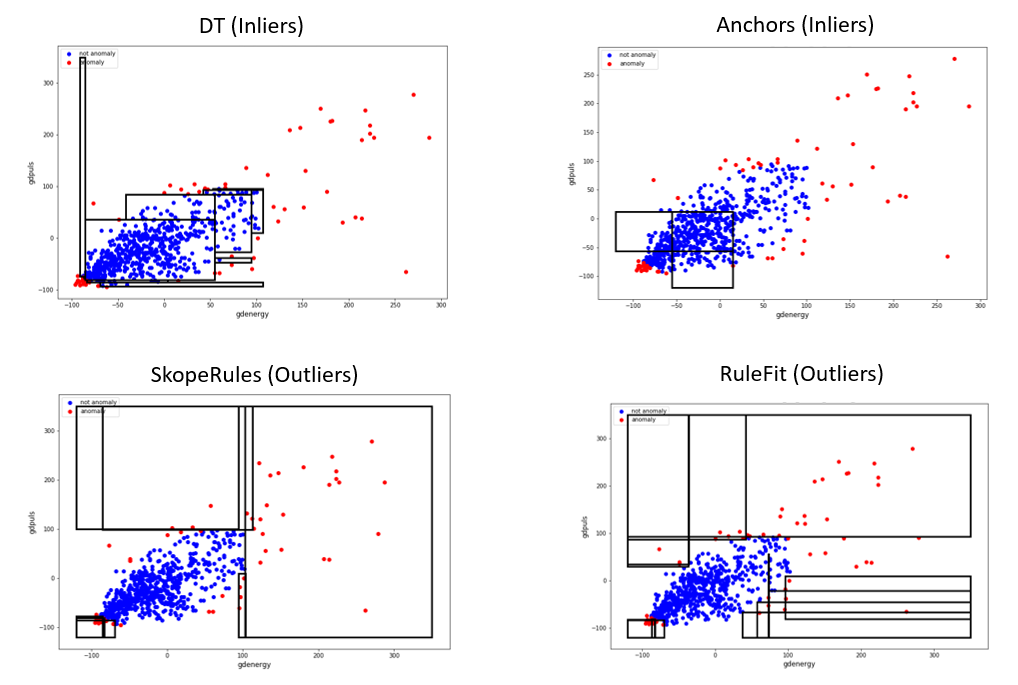
\includegraphics[width=0.9 \columnwidth]{figures/chapter4_RuleExtraction/RuleExtractionOther.PNG}
  \end{tabular} 
  \caption{Visualizations for the rules extracted over D1 with RBF kernel with DT and Anchors (for inliers) and SkopeRules and RuleFit (for outliers). \label{fig:ch4-evaluation-img-other-2D}}
\end{figure}


The results appear in \hyperref[table:annex-rule-extraction-xai-metrics-H3]{Table} \ref{table:annex-rule-extraction-xai-metrics-H3}. Here, we see how \textbf{KM\_split is generally better for every metric except for the ones related to \textit{comprehensibility}}. In particular, KM\_split is able to significantly cover more data points from the target class with P@1 rules (per\_p1) than any of the other methods, and also yields rules that have better coverage (p1\_coverage) than FRL and brlg. However, the mean coverage per rule compared to the other methods is not significantly different. Regarding \textit{stability}, KM\_split outperforms brlg, but brlg has a better result in terms of \textit{diversity}. KM\_split improves FRL and Anchors in \textit{stability}, and DT in \textit{diversity}. Finally, considering the general metric, KM\_split has significantly better results than any of the other methods, with the exception of DT, where it does not show significant differences. Considering KM\_keep, the results are similar, as shown in \hyperref[table:annex-rule-extraction-xai-metrics-H3-2]{Table} \ref{table:annex-rule-extraction-xai-metrics-H3-2}. One difference is that since KM\_keep has a better general metric than KM\_split, it is also able to significantly outperform DT in that aspect. Also, KM\_keep is not outperformed in terms of \textit{diversity} by brlg, as opposed to KM\_split.

As a conclusion, we see that both the solution of \parencite{nunez2002rule} with K-Means++ (and with the modification for generating rules for categorical features), together with the variations considered in this chapter (for also K-Means++ as clustering method) yield similar results in terms of most of the XAI metrics considered in this chapter for explaining the results of a OCSVM anomaly detection model using P@1 rules. The results in terms of \textit{comprehensibility} (number of rules) are influenced depending on the type of kernel used, and whether they are explaining inliers or outliers. Finally, comparing these techniques with other rule extraction methods, we saw a \textbf{trade-off between \textit{comprehensibility} and the remaining XAI metrics}. The clustering-based rule extraction techniques used in this chapter are able to explain better, using P@1 rules, the results of a OCSVM model (considering the data sets and kernels of this chapter) in terms of \textit{representativeness}, \textit{stability} and \textit{diversity}, but in exchange of \textit{comprehensibility}, which is penalized.


\section{Conclusion}\label{sec:RuleExtractionConclusion}
In this chapter, we presented variations over existing rule extraction XAI algorithms, as well as specific XAI metrics, for generating and evaluating explanations within the context of unsupervised ML for anomaly detection.
First, we highlighted that even though rule extraction XAI methods can theoretically be applied over unsupervised ML for anomaly detection (since the output is similar to that of a supervised binary classifier), there are specific considerations that should be taken into account, and there is a lack of research regarding that. Among these considerations, we find that there is commonly a great data imbalance between the two classes, there is normally a need to explain only one of the classes (outliers) in a counterfactual way, and the explanations must be P@1 within several use cases. Thus, some rule extraction techniques may be more suitable than others within this context. 
Because of that, we proposed \textbf{SVM+Prototypes reloaded}, an algorithm for generating both post-hoc global and local counterfactual rule-based explanations that are model agnostic.  This algorithm is a variant from a previous one within the literature, and comes with two alternative methods.
However, for evaluating and finding the best rule extraction technique in every context, we need quantitative metrics that measure the quality of the explanations against several aspects. Regarding this, we proposed several \textbf{XAI metrics} for measuring different aspects of the explanations generated. In particular, for measuring their \textit{comprehensibility, representativeness, stability and diversity}. For the particular cases of \textit{stability} and \textit{diversity}, we proposed novel metrics through \textbf{StabilityScore} and \textbf{DiversityScore} for measuring these aspects. We also discuss on the importance of combining all the metrics into one in order to simplify the analyses (although this is not necessary in some use cases).
Finally, we propose a framework that standardizes the output of the different rule extraction techniques in order to carry out the evaluation through those metrics. This framework also prunes the rules, eliminating redundant ones.
With that, we can consider our hypothesis \textbf{H1} (\hyperref[sec:Hypotheses]{Section} \ref{sec:Hypotheses}) validated by both mathematically justifying XAI metrics, as well as evaluating them over different data sets in order to quantify explanation differences between rule extraction methods within the context of unsupervised anomaly detection.